% IF YOU CAN SEE THIS GO CONTRIBUTE >:(

\documentclass[letterpaper, 8pt]{extarticle}
\usepackage{amssymb,amsmath,amsthm,amsfonts}
\usepackage{multicol,multirow}
\usepackage{calc}
\usepackage{ifthen}
\usepackage[landscape]{geometry}
\usepackage[colorlinks=true,citecolor=blue,linkcolor=blue]{hyperref}

\usepackage{booktabs}
\usepackage{ulem}
\usepackage{enumitem}
\usepackage{tabulary}
\usepackage{graphicx}
\usepackage{siunitx}
\usepackage{tikz}
\usepackage{derivative}
\usepackage{svg}
\usepackage{listings}
\usepackage{setspace}
\usepackage{listings}
\usepackage{xcolor}
\usepackage{courier}
\usepackage{syntax}
\usepackage{mathpartir}

% minimal line spacing
\setstretch{0.1}

% set borders (experimentally determined to minimize cutoff and maximize space on school printers)
\geometry{top=.25in,left=.25in,right=.25in,bottom=.35in}

% make figures work better in multicol
\newenvironment{Figure}
{\par\medskip\noindent\minipage}
{\endminipage\par\medskip}

\pagestyle{empty} % clear page

% rewrite section commands to be smaller
\makeatletter
\renewcommand{\section}{\@startsection{section}{1}{0mm}%
                                {-1explus -.5ex minus -.2ex}%
                                {0.5ex plus .2ex}%x
                                {\normalfont\normalsize\bfseries}}
\renewcommand{\subsection}{\@startsection{subsection}{2}{0mm}%
                                {-1explus -.5ex minus -.2ex}%
                                {0.5ex plus .2ex}%
                                {\normalfont\small\bfseries}}
\renewcommand{\subsubsection}{\@startsection{subsubsection}{3}{0mm}%
                                {-1ex plus -.5ex minus -.2ex}%
                                {1ex plus .2ex}%
                                {\normalfont\tiny\bfseries}}
\makeatother
\setcounter{secnumdepth}{0} % disable section numbering


% disable indenting
\setlength{\parindent}{0pt}
\setlength{\parskip}{0pt plus 0.5ex}

% Custom siunitx defs
\DeclareSIUnit\noop{\relax}
\NewDocumentCommand\prefixvalue{m}{%
\qty[prefix-mode=extract-exponent,print-unity-mantissa=false]{1}{#1\noop}
}

% Shorthand definitions
\newcommand{\To}{\Rightarrow}
\newcommand{\ttt}{\texttt}
\newcommand{\ra}{\rightarrow}

% condense itemize & enumerate
\let\olditemize=\itemize \let\endolditemize=\enditemize \renewenvironment{itemize}{\olditemize \itemsep0em}{\endolditemize}
\let\oldenumerate=\enumerate \let\endoldenumerate=\endenumerate \renewenvironment{enumerate}{\oldenumerate \itemsep0em}{\endoldenumerate}
\setlist[itemize]{noitemsep, topsep=0pt, leftmargin=*}
\setlist[enumerate]{noitemsep, topsep=0pt, leftmargin=*}

\title{3N03}

\begin{document}
\raggedright
\tiny

% make listings look nicer
\lstset{
	tabsize = 2, %% set tab space width
	showstringspaces = false, %% prevent space marking in strings, string is defined as the text that is generally printed directly to the console
	basicstyle = \tiny\ttfamily, %% set listing font and size
	breaklines = true, %% enable line breaking
	numberstyle = \tiny,
	postbreak = \mbox{\textcolor{red}{\(\hookrightarrow\)}\space}
}

\begin{center}
	{\textbf{3N03 Final Cheatsheet}} \\
\end{center}
% set column spacing rules
\setlength{\premulticols}{1pt}
\setlength{\postmulticols}{1pt}
\setlength{\multicolsep}{1pt}
\setlength{\columnsep}{2pt}
\begin{multicols*}{4}

	\section{Network Fundamentals}
	\textbf{Network:} Collection of devices interconnected by a single technology (internet) \\
	\subsection{Network Uses}
	\textbf{Business Applications:} Resource/info sharing, communication, client-server model \\
	\textbf{Home Applications:} Peer-to-peer model \\
	\textbf{Mobile Users:} Wireless connectivity

	\subsection{E-Commerce Types}
	B2C: Business to Consumer \\
	B2B: Business to Business \\
	G2C: Government to Consumer \\
	C2C: Consumer to Consumer \\
	P2P: Peer to Peer

	\subsection{Social Issues}
	Network Neutrality, Content ownership, Anonymity \& Censorship, Privacy, Info Theft

	\subsection{Network Scales}
	\textbf{PAN:} Personal (Bluetooth) \\
	\textbf{LAN:} Local (Office) \\
	\textbf{MAN:} Metropolitan (City) \\
	\textbf{WAN:} Wide (Country/ISP (Internet Service Provider), a company). Serve as modern internet backbone. \\
	\textbf{Internet:} Network of networks (Planet)
	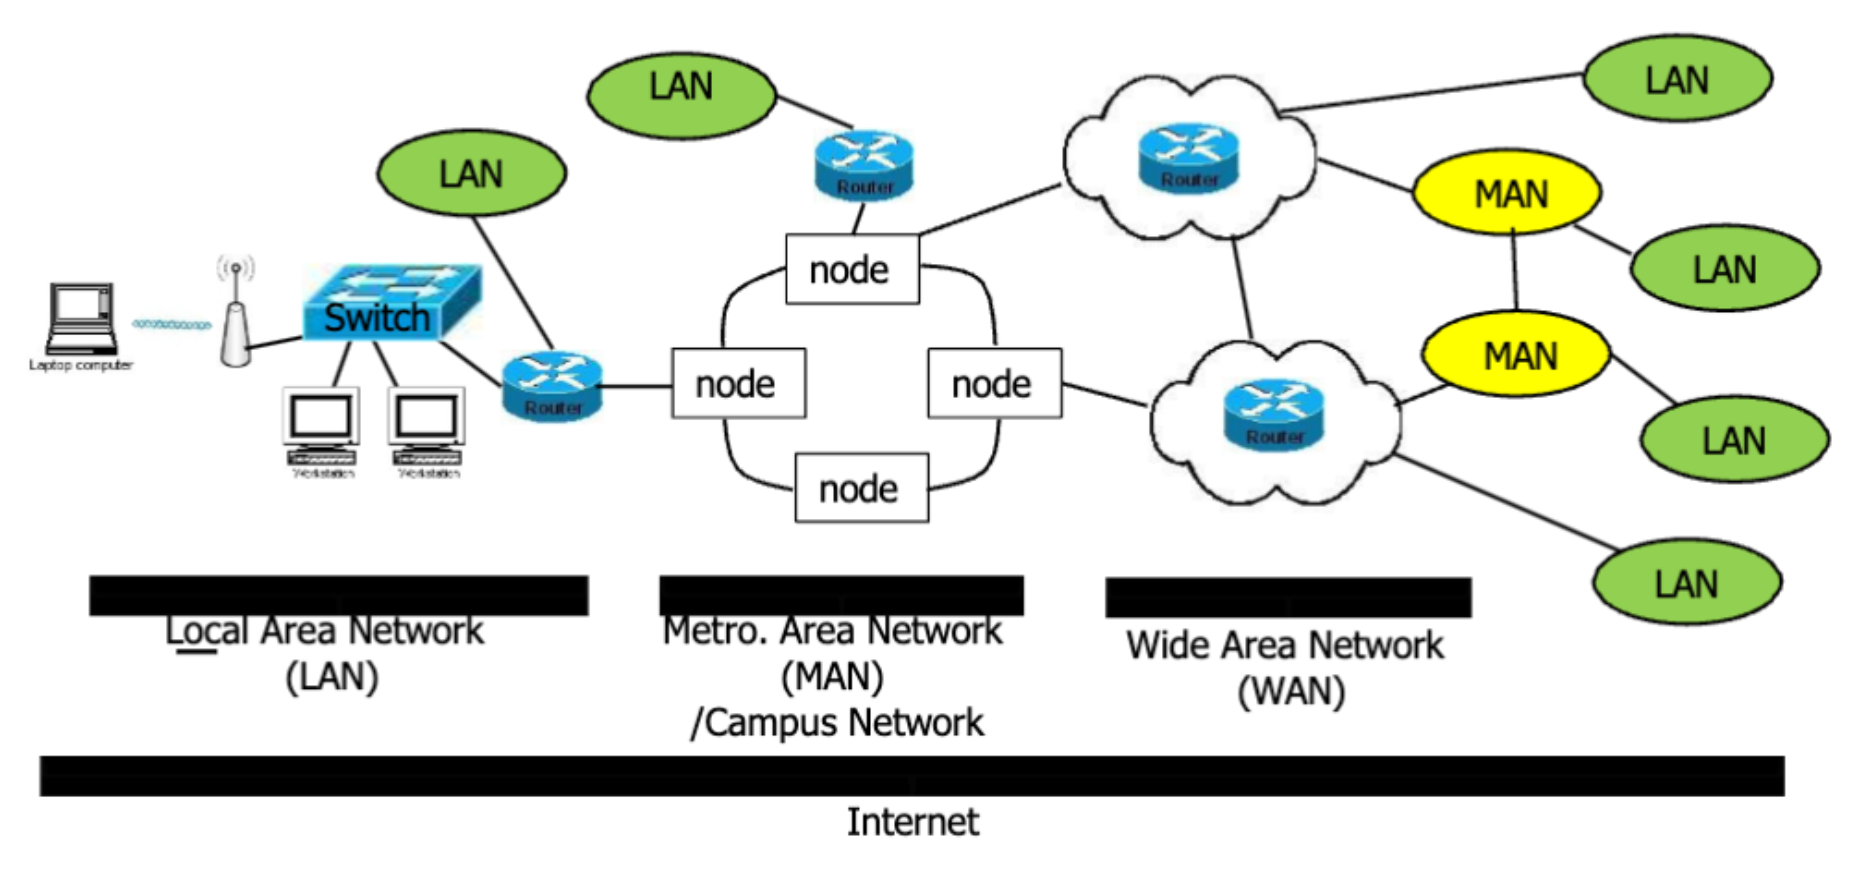
\includegraphics[width=\linewidth]{SCR-20250416-trqu.png}

	\subsection{Connection Types}
	\textbf{Internetwork:} Network of smaller networks \\
	\textbf{Internet:} Set of all connected networks \\
	\textbf{Gateway:} Device transferring data between layers \\
	\textbf{Low-Level Gateways:}
	\begin{itemize}
		\item Operate at the lower layers of the network protocol
		\item More limited in functionality
		\item Cannot effectively connect different types of networks
		\item *Focus on basic data transmission*
	\end{itemize}
	\textbf{High-Level Gateways:}
	\begin{itemize}
		\item Operate at higher layers of the protocol stack (application layer)
		\item Very specific in their function
		\item Limited to particular applications or services
		\item Example: An email gateway that only handles email traffic
		\item *While powerful for specific uses, they're too specialized for general network connectivity*
	\end{itemize}
	\textbf{Best Mid-level Gateways}
	\begin{itemize}
		\item "just right"
		\item Represented by routers, which operate at the network layer
		\item Provide the optimal balance between functionality and flexibility
		\item Can effectively route packets between different networks
		\item \textit{Handle most common networking needs}
		\item Can connect different types of networks while maintaining good performance
	\end{itemize}
	\textbf{Router:} Gateway for network layer information

	\subsection{Transmission Technology}
	\begin{itemize}
		\item broadcast links - communication channel shared by all machines in network
		\item point-to-point - direct connection between two machines
		\item packet - small unit of data sent over a network.
	\end{itemize}

	\section{Layered Network Models}
	Each layer implements a service. Layering provides encapsulation, where each layer adds its own header to data.

	\subsection{Design Issues}
	\begin{itemize}
		\item Reliability/failure handling
		\item Network growth capability
		\item Resource allocation
		\item Security against threats
	\end{itemize}

	\subsection{Layer services}
	\textbf{Vertical:} services for uni directional communication from top layer to bottom layer, like a gateway \\
	\textbf{Horizontal:} protocols for communication between same layers
	\textbf{connection oriented:} set up for ongoing use, torn down afterwords
	\textbf{connectionless:} separately and temporary handled messages

	\subsection{OSI Model}
	Open Systems Interconnection. Makes essential concepts explicit (services, interfaces, protocols). \\
	\textbf{7. Application:} Network apps, end-user access, protocols (FTP, SMTP, HTTP) \\
	\textbf{6. Presentation:} Data interpretation/formatting \\
	\textbf{5. Session:} provides locality for different transport streams to not confuse individual streams. Estabashing a method of communicatino. \\
	\textbf{4. Transport:} Process-to-process data transfer, segmentation, reliability (TCP, UDP) \\
	\textbf{3. Network:} packet routing between networks (IP) \\
	\textbf{2. Data Link:} raw bit collection, physical addressing, unit of data in frames \\
	\textbf{1. Physical:} Raw bit transmission (cables, signals)
	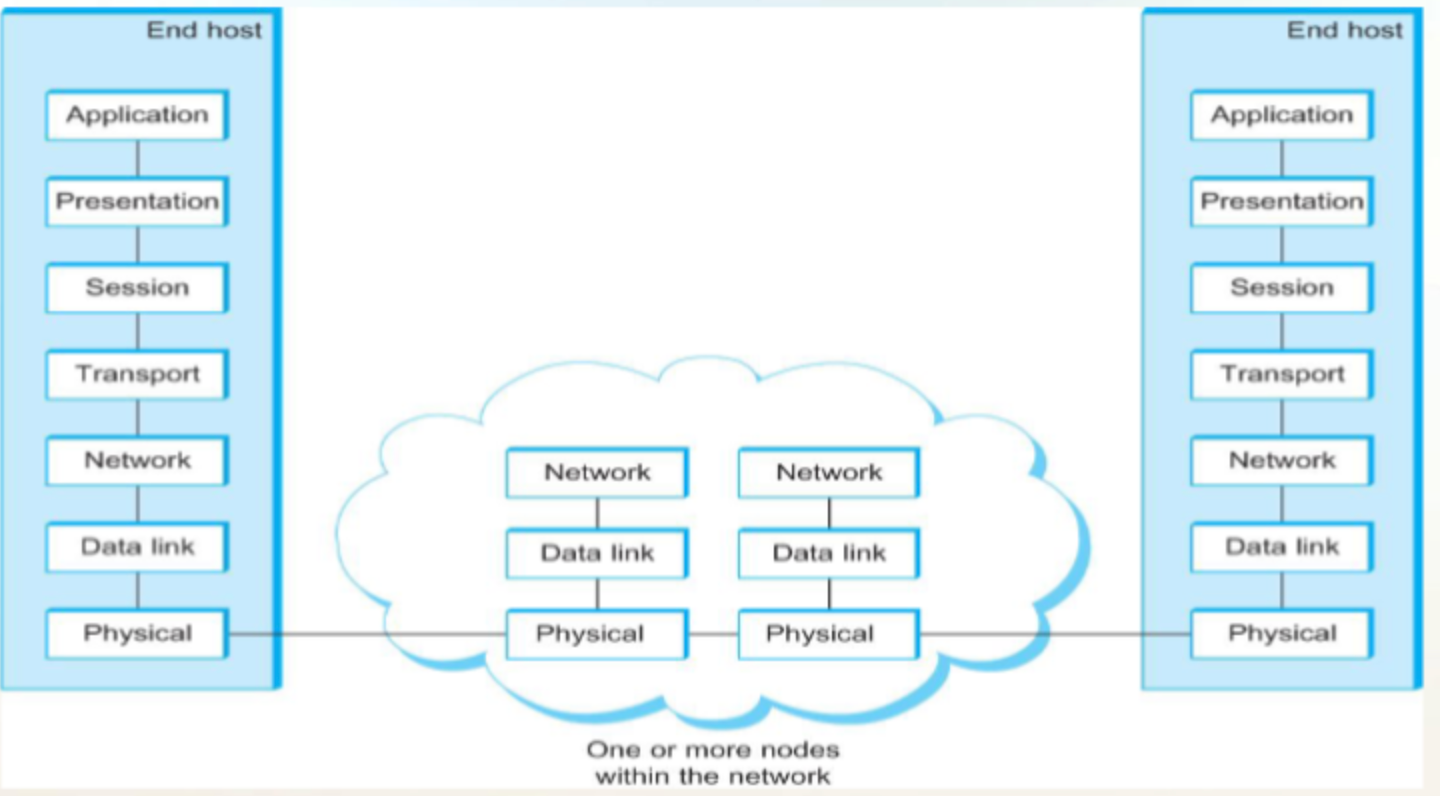
\includegraphics[width=\linewidth]{SCR-20250416-ucdl.png}

	\subsection{TCP/IP Model}
	More specific to the internet, heavily relies on protocols, whereas OSI model is more generalized. \\
	\textbf{4. Application:} TELNET, FTP, SMTP, DNS, HTTP, RTP \\
	\textbf{3. Transport:} TCP (reliable, connection-oriented), UDP (unreliable, connectionless) \\
	\textbf{2. Internet:} IP packet delivery, multi-network connection support. \\
	\textbf{1. Link:} implemented by combinatino of hardware (ethernet, fiberoptics, etc).
	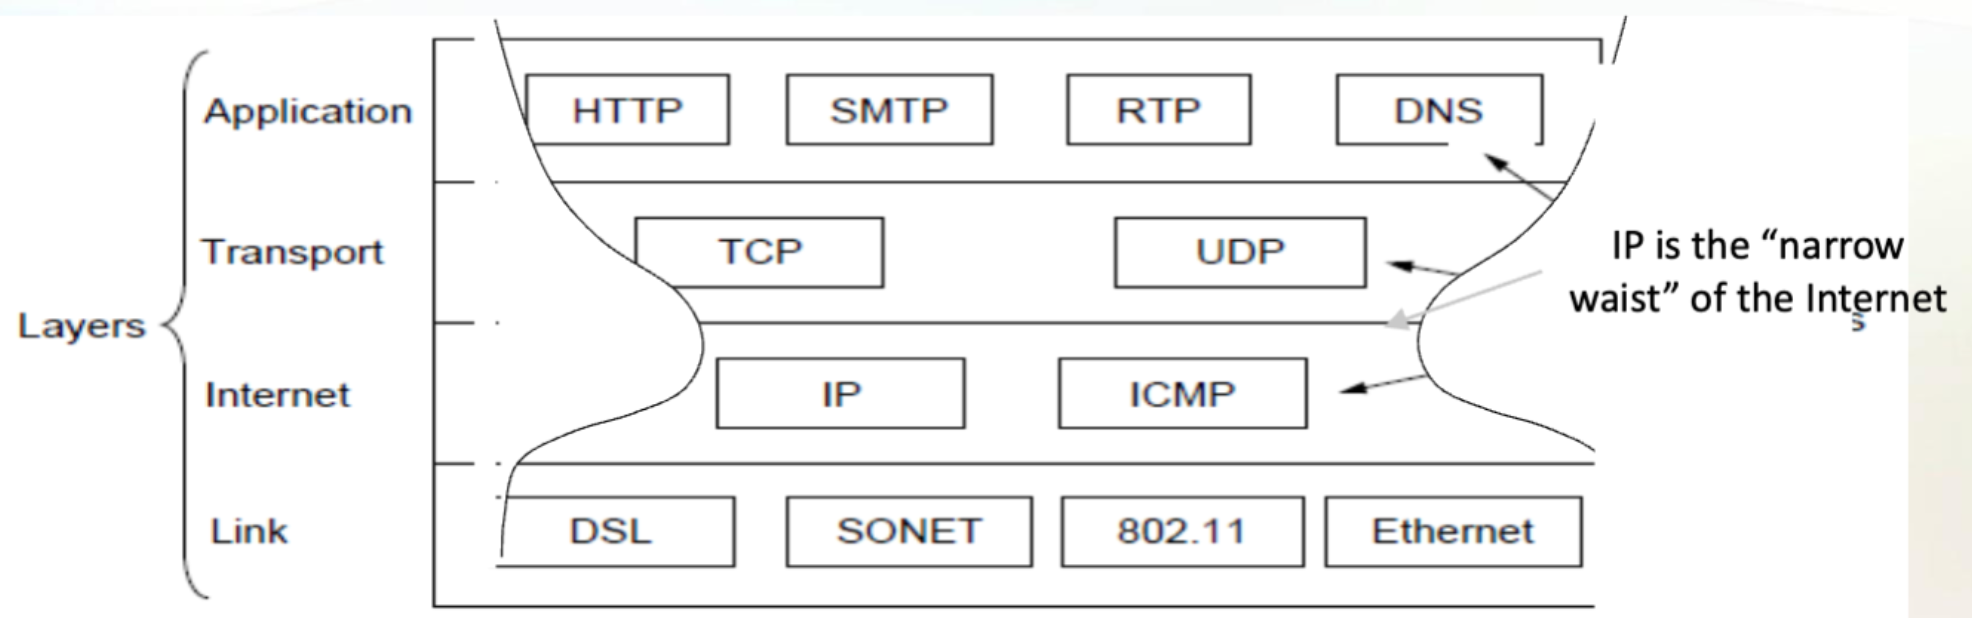
\includegraphics[width=\linewidth]{SCR-20250416-udrs.png}

	\section{Data Transmission}
	\textbf{Packet Transmission Delay:} $\frac{L}{R}$ (Length/Rate) \\
	\textbf{Store \& Forward:} Full packet received before forwarding, end-to-end delay = $2\frac{L}{R}$

	\subsection{Network Core Functions}
	\textbf{Routing:} Determining packet paths \\
	\textbf{Forwarding:} Moving packets between router interfaces

	\section{Application Layer}
	\subsection{Architectures}
	\textbf{Client-Server:}
	\begin{itemize}
		\item Clients communicate with server
		\item Server: permanent IP, always-on
		\item Clients: dynamic IP, intermittent connectivity
	\end{itemize}

	\textbf{Peer-to-Peer (P2P):}
	\begin{itemize}
		\item Minimal server reliance
		\item Direct end-system communication
		\item Self-scaling with new peers
		\item Challenges: security, performance, management
	\end{itemize}

	\subsection{Application Requirements}
	\textbf{Data Transfer:} Reliability needs \\
	\textbf{Timing:} Delay sensitivity \\
	\textbf{Throughput:} Bandwidth requirements \\
	\textbf{Security:} Encryption, authentication

	\subsection{Transport Protocols}
	A protocol is a set of rules governing the format and meaning of the packets or messages that are exchanged. Protocols implement the services. \\
	\textbf{TCP Service:}
	\begin{itemize}
		\item Reliable transport
		\item Flow control
		\item Congestion control
		\item Connection-oriented
		\item No timing/throughput guarantees
		\item No built-in security
	\end{itemize}

	\textbf{UDP Service:}
	\begin{itemize}
		\item Unreliable data transfer
		\item No guarantees
		\item Low overhead
	\end{itemize}

	\textbf{Securing TCP:} SSL (Secure Socket Layer) at application layer

	\subsection{HTTP Protocol}
	\textbf{Properties:}
	\begin{itemize}
		\item Client/server model
		\item TCP on port 80
		\item Stateless
		\item Non-Persistent: One object per connection
		\item Persistent: Multiple objects per connection
	\end{itemize}

	\textbf{Request Message:}
	\begin{itemize}
		\item ASCII format
		\item Request line, header lines, empty body
	\end{itemize}
	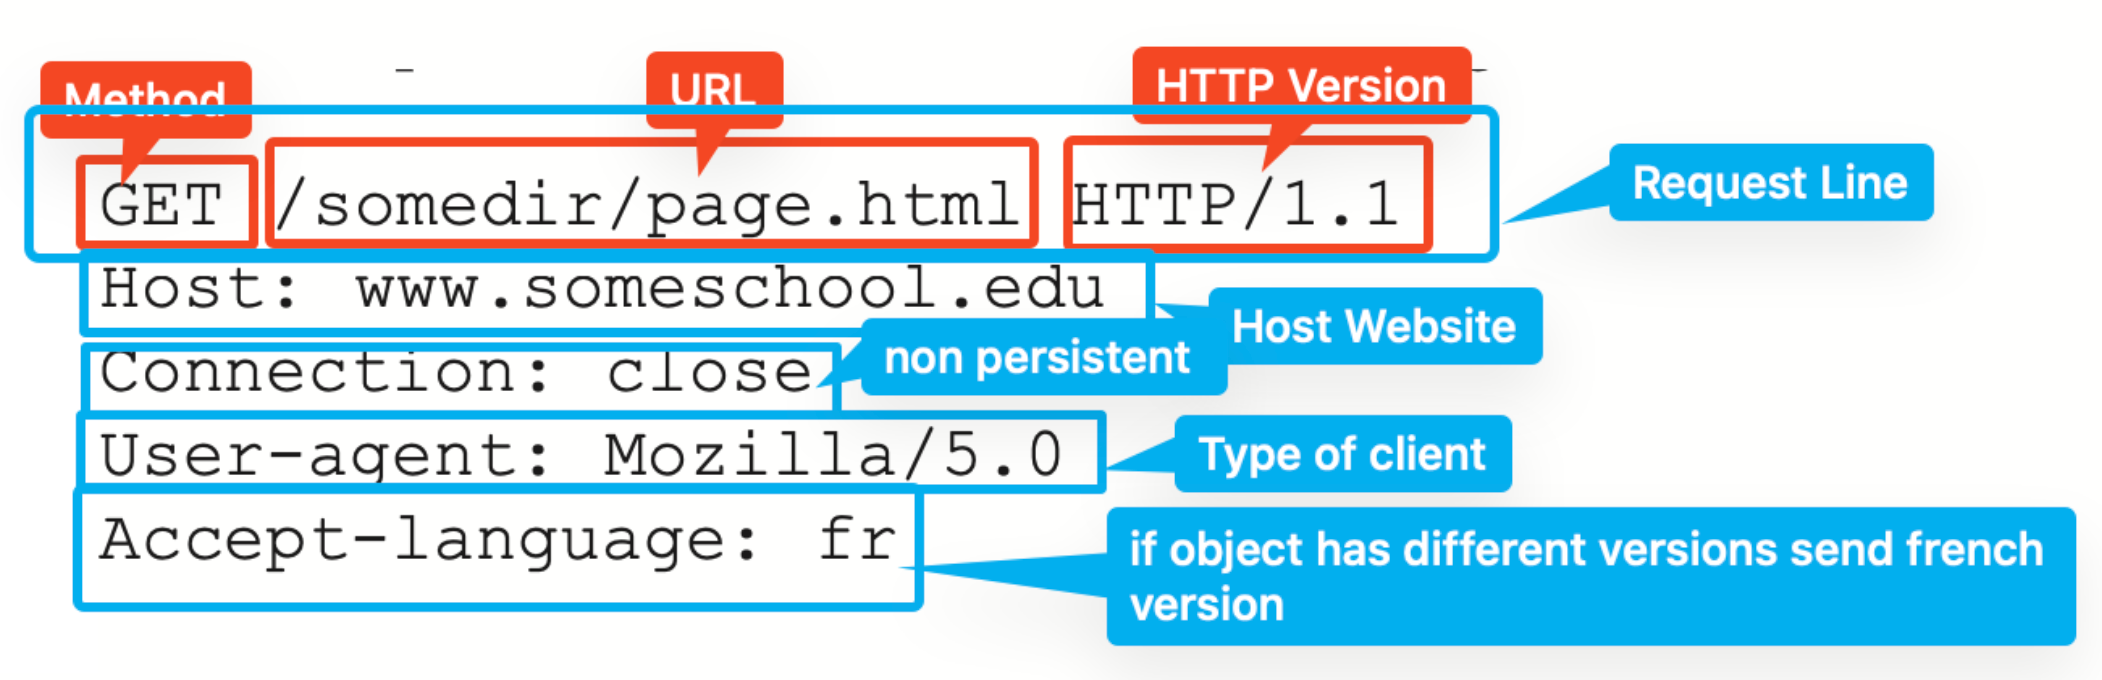
\includegraphics[width=\linewidth]{http-request.png}

	\textbf{Response Message:}
	\begin{itemize}
		\item ASCII format
		\item Status line, header lines, data
	\end{itemize}
	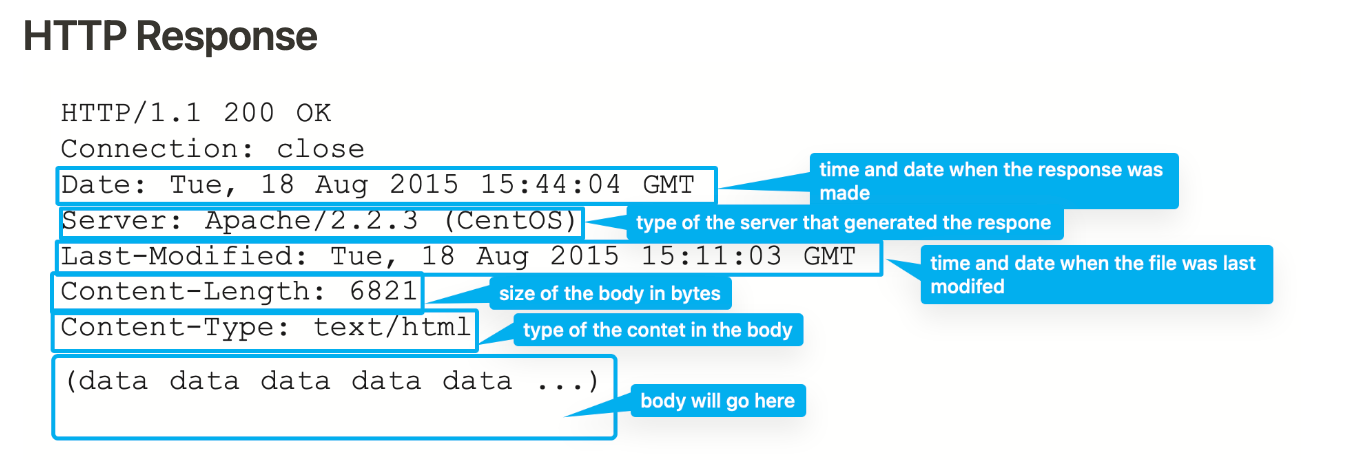
\includegraphics[width=\linewidth]{http-response.png}

	\textbf{Status Codes:}
	\begin{itemize}
		\item 1xx: Informational
		\item 2xx: Success (200 OK)
		\item 3xx: Redirection (301 Moved)
		\item 4xx: Client Error (404 Not Found)
		\item 5xx: Server Error
	\end{itemize}

	\textbf{Services}
	\begin{itemize}
		\item GET: Retrieve data
		\item HEAD: read a webpage's header
		\item POST: Create new data
		\item PUT: update existing data
		\item DELETE: remove data
		\item TRACE: echo incoming request
		\item CONNECT: connect through a proxy
		\item OPTIONS: query options for a page
	\end{itemize}

	\subsection{Cookies}
	\begin{itemize}
		\item Stateful client/server interactions
		\item saves user data and activity in servers
		\item sent via clients/browsers
		\item Cookie header line in [[http]] response messag
		\item Cookie header line in [[http]] request message
		\item cookie file stored locally, managed by user client
		\item backend database at the website
		\item Uses
		      \begin{itemize}
			      \item authorization
			      \item shopping carts
			      \item recommendations
			      \item user session state
		      \end{itemize}
	\end{itemize}

	\subsection{Web Cache/Proxy}
	Browser connects to proxy not web server; reduces latency, proxy acts as client+server

	\subsection{MIME type}
	Multipurpose Internet Mail Extension. Encoding rules.
	% \begin{table}[!htbp]
	% 	\tiny
	% 	\setlength{\tabcolsep}{2pt}
	% 	\centering
	% 	\caption{Multipurpose Internet Mail Extension: Encoding Rules}
	% 	\begin{tabular}{|p{2cm}|p{3cm}|}
	% 		\hline
	% 		\textbf{Header}            & \textbf{Meaning}                                     \\
	% 		\hline
	% 		MIME-Version:              & Identifies the MIME version                          \\
	% 		\hline
	% 		Content-Description:       & Human-readable string telling what is in the message \\
	% 		\hline
	% 		Content-Id:                & Unique identifier                                    \\
	% 		\hline
	% 		Content-Transfer-Encoding: & How the body is wrapped for transmission             \\
	% 		\hline
	% 		Content-Type:              & Type and format of the content                       \\
	% 		\hline
	% 	\end{tabular}
	% \end{table}
	% ------------------------- MIME header fields -------------------------
	% ---------------- MIME header fields ----------------
	\textbf{MIME Header Fields}

	{\renewcommand{\arraystretch}{12}%  <‑‑‑ added
		\begin{tabulary}{\linewidth}{@{}LL@{}} \toprule
			\textbf{Header} & \textbf{Meaning} \\ \midrule
			MIME-Version            & Identifies the MIME version \\
			Content-Description     & Human‑readable string telling what is in the message \\
			Content-Id              & Unique identifier \\
			Content-Transfer-Encoding & How the body is wrapped for transmission \\
			Content-Type            & Type and format of the content \\
			\bottomrule
		\end{tabulary}
	} % <‑‑‑ closes the local arraystretch change

	% ---------------- MIME content types ----------------
	\textbf{MIME Content Types}

	{\renewcommand{\arraystretch}{12}%  <‑‑‑ added
		\begin{tabulary}{\linewidth}{@{}LLL@{}} \toprule
			\textbf{Type} & \textbf{Example subtypes} & \textbf{Description} \\ \midrule
			text        & plain, html, xml, css                     & Text in various formats \\
			image       & gif, jpeg, tiff                           & Pictures \\
			audio       & basic, mpeg, mp4                          & Sounds \\
			video       & mpeg, mp4, quicktime                      & Movies \\
			model       & vrml                                      & 3D model \\
			application & octet‑stream, pdf, javascript, zip        & Data produced by applications \\
			message     & http, rfc822                              & Encapsulated message \\
			multipart   & mixed, alternative, parallel, digest      & Combination of multiple types \\
			\bottomrule
		\end{tabulary}
	}




	\subsection{Email Architecture}
	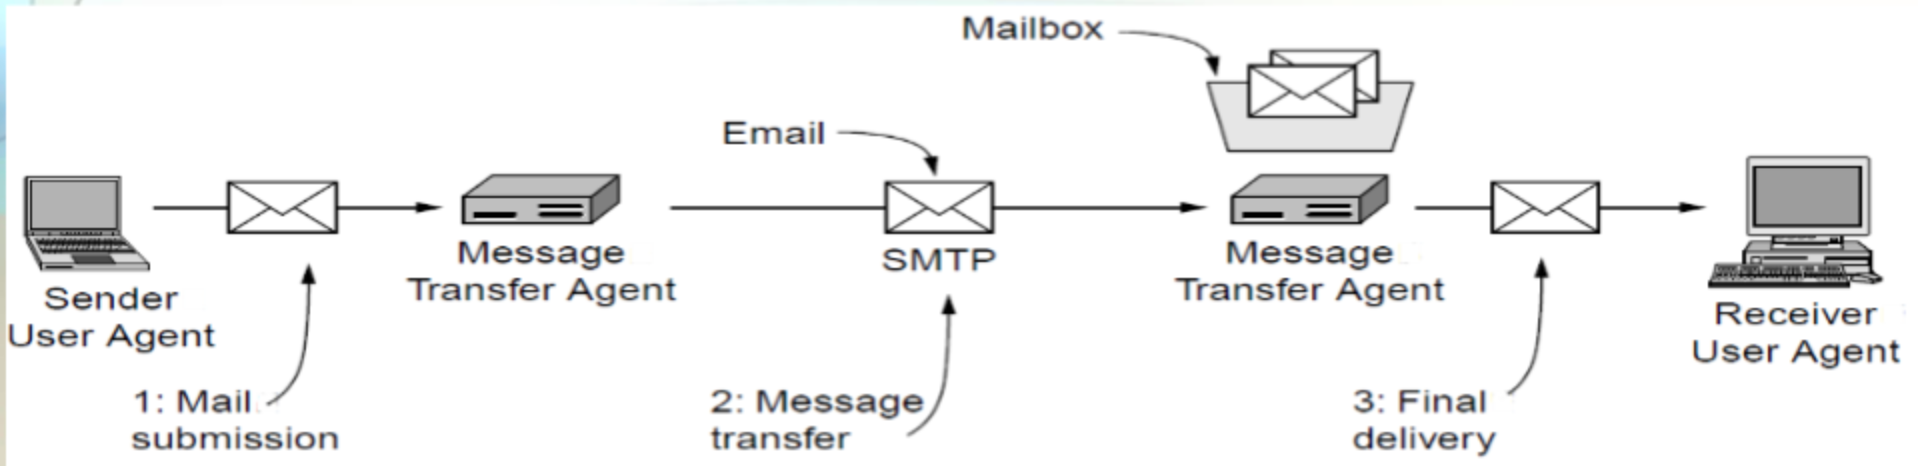
\includegraphics[width=\linewidth]{SCR-20250417-bixw.png}
	\textbf{Components:}
	\begin{itemize}
		\item User Agents: For reading and sending email. Mail clients (Outlook, Apple Mail)
		\item Mail Servers: Mailbox and message queue
	\end{itemize}

	\textbf{SMTP (Simple Mail Transfer Protocol):}
	\begin{itemize}
		\item Client-server between mail servers
		\item Persistent TCP (port 25)
		\item Phases: Handshake, Transfer, Closure
		\item "Push" protocol (sending)
	\end{itemize}

	\textbf{Mail Access Protocols:}
	\begin{itemize}
		\item POP3: Download from server (port 110)
		      \begin{itemize}
			      \item Authorization, Transaction, Update
			      \item Download-and-Delete or Download-and-Keep
			      \item Stateless across sessions
			      \item No remote folders
		      \end{itemize}
		\item IMAP: Internet message Access Protocol is used for final delivery. Listens to port 143. More secure and more features than POP3.
	\end{itemize}

	\subsection{DNS (Domain Name System)}
	Hierarchical domain based naming scheme with a database to implement it. Maps hostname to IP addresses, called \textbf{resolution}. \textbf{Name server} is in charge of a select group of domains.

	\textbf{How it works}
	\begin{enumerate}
		\item application program has hostname, passes it to resolver
		\item resolver passes *hostname* to DNS server
		\item DNS server returns IP address, sent as UDP packets
	\end{enumerate}
	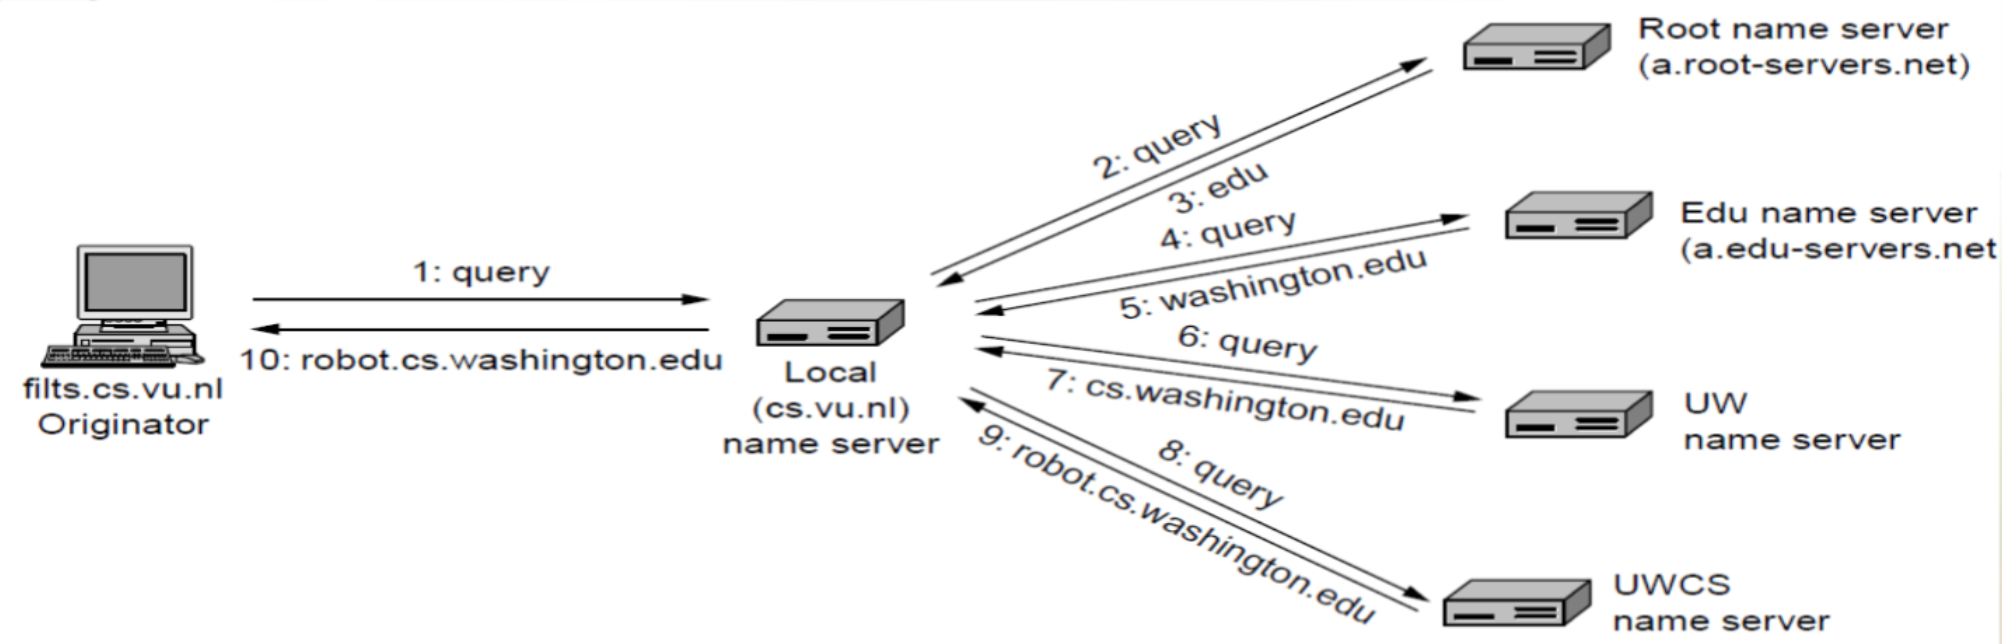
\includegraphics[width=\linewidth]{SCR-20250417-brck.png}

	\textbf{Hierarchy:}
	\begin{itemize}
		\item ICANN (Internet Corporation for Assigned Names and Numbers)
		\item 250 top level domains, generics and one per country
		\item top level domains divided into subdomains
	\end{itemize}
	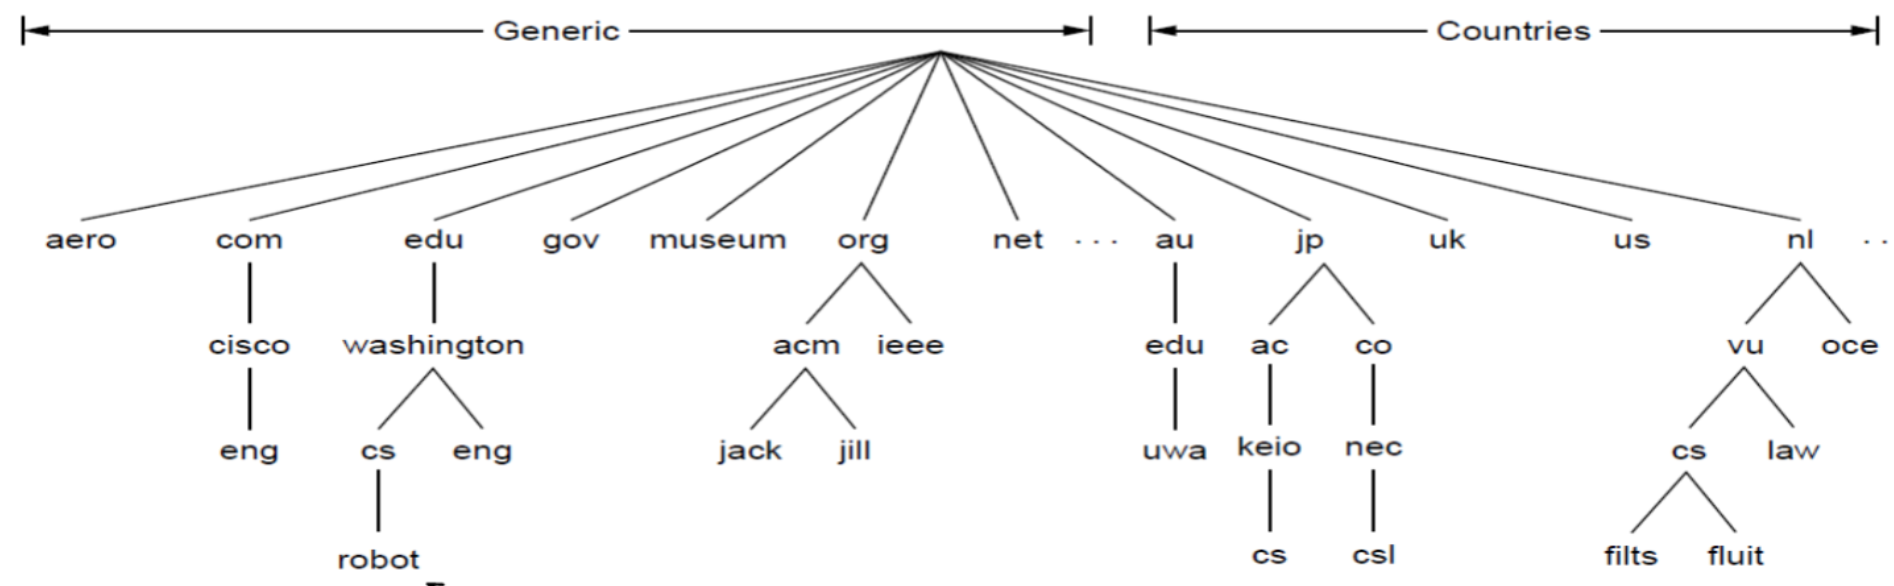
\includegraphics[width=\linewidth]{SCR-20250417-bplh.png}

	\textbf{Vulnerabilities:}
	\begin{itemize}
		\item DDoS attacks
		\item Redirect attacks (MITM, poisoning)
		\item Using DNS for DDoS amplification
	\end{itemize}

	\section{Transport Layer}
	\textbf{Functions:}
	\begin{itemize}
		\item Communication between applications where from sender process the reciever process is on the same device.
		\item Implemented in end systems (not routers)
		\item Segments application messages and pass to network layer
		\item Routers read network layer datagrams not transport layer segments
	\end{itemize}

	\subsection{Multiplexing/Demultiplexing}
	\textbf{Process:}
	\begin{itemize}
		\item ensures communication between processes/host on sender\&reciever in transport layer/network layer
		\item On client side ts layer assigns src/dest ports to segments when multiplexing
		\item On reciever side, ts layer uses dest port to demultiplex segments into correct sockets
	\end{itemize}

	\textbf{Protocols:}
	\begin{itemize}
		\item TCP sockets: (source IP, source port, dest IP, dest port) tuple so based on source different sockets are made
		\item UDP sockets: (dest IP, dest port) tuple so the socket doesn't differentiate between different clients and sends all data to the same process
	\end{itemize}



	\subsection{Reliable Data Transfer}
	\textbf{Error types:}
	\begin{itemize}
		\item Corruption (packet received incorrectly)
		\item Loss (packet never arrives)
	\end{itemize}

	\subsection{UDP Characteristics}
	\textbf{Features:}
	\begin{itemize}
		\item Connectionless
		\item No handshaking
		\item Each segment handled independently
		\item No congestion control
		\item Has checksum for error detection
	\end{itemize}


	\subsection{TCP Characteristics}
	\textbf{Features:}
	\begin{itemize}
		\item Full-duplex service
		\item Point-to-point (single sender, single receiver)
		\item Connection-oriented with handshaking
		\item Reliable, ordered byte stream
		\item Flow control
		\item Congestion control
	\end{itemize}

	\textbf{Segment Structure:}
	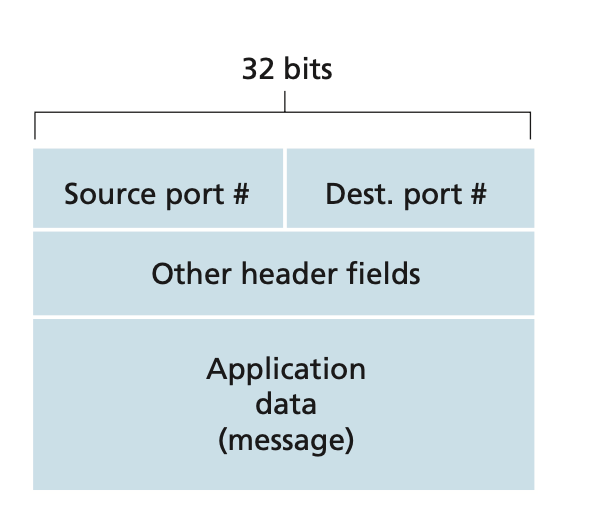
\includegraphics[width=\linewidth]{segment-packet.png}
	\begin{itemize}
		\item Data field (limited by MSS)
		\item 32-bit sequence number
		\item 32-bit acknowledgment number
		\item 16-bit receive window
		\item 4-bit header length
		\item 6-bit flag field
		\item Options field
	\end{itemize}

	\subsection{TCP interaction example}
	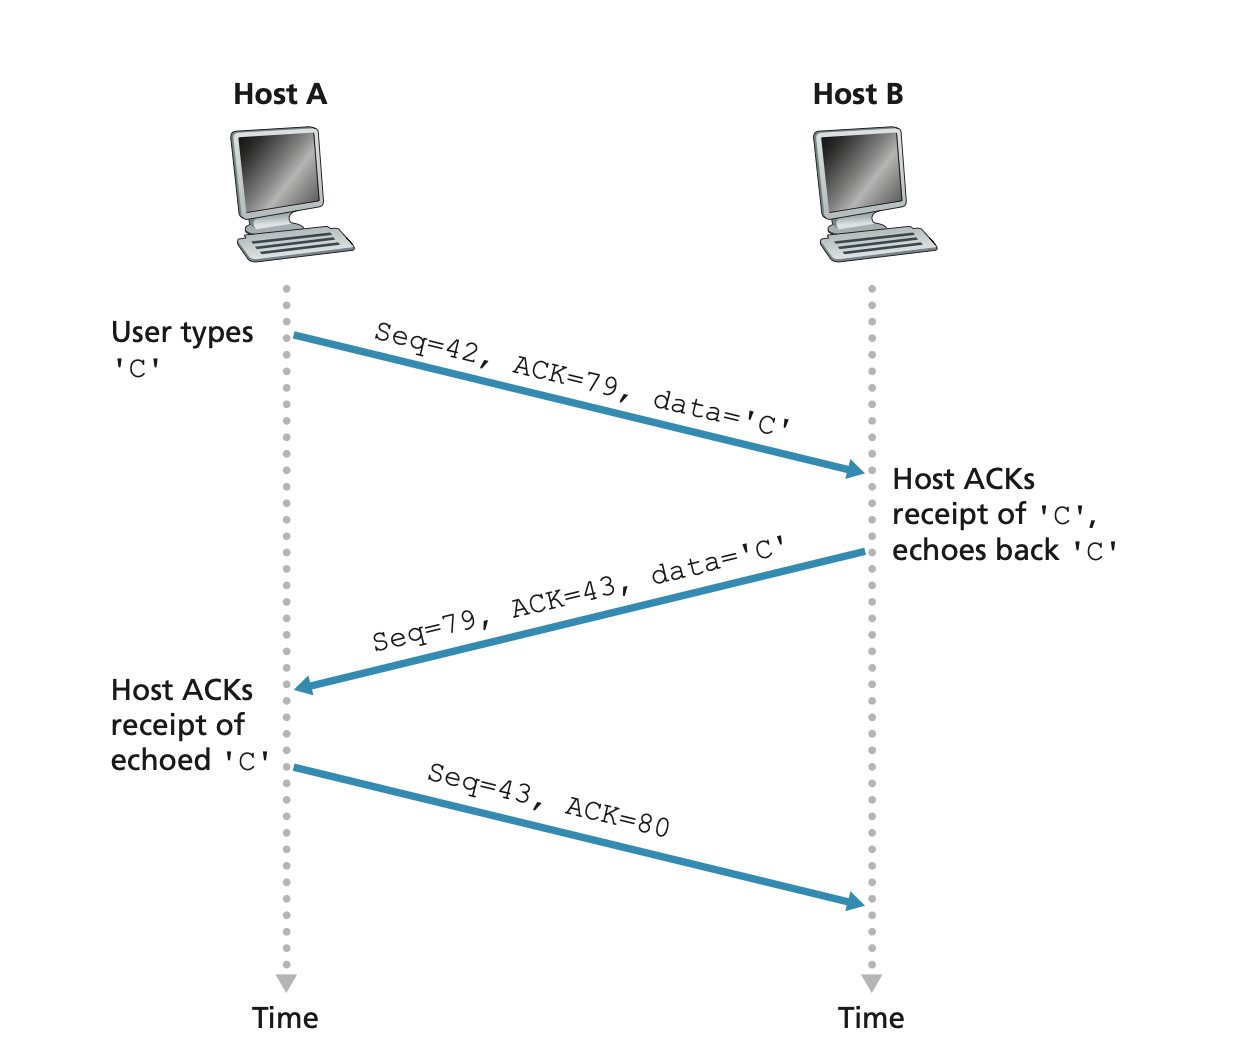
\includegraphics[width=\linewidth]{telnet.png}
	\subsection{UDP Checksum Calculation}
	\textbf{Process:}
	\begin{itemize}
		\item Covers UDP header + data + pseudo-header
		\item Sender: Sum all 16-bit words, wrap when overflow, negate the result
		\item Receiver: Sum all 16-bit words including checksum, result should be all 1's
	\end{itemize}

	\textbf{Example:}
	\begin{itemize}
		\item Data: 0x1234, 0x5678, 0xABCD
		\item Sum: 0x1234 + 0x5678 = 0x68AC
		\item Sum: 0x68AC + 0xABCD = 0x11479 (overflow)
		\item Wrap around: 0x1479 + 0x0001 = 0x147A
		\item 1's complement: 0xFFFF - 0x147A = 0xEB85
		\item Checksum field: 0xEB85
		\item Receiver adds: 0x1234 + 0x5678 + 0xABCD + 0xEB85 = 0x1FFFE
		\item Wrap around: 0x1FFFE + 0x0001 = 0xFFFF (all 1's)
	\end{itemize}


	\section{Socket Programming}
	\textbf{Socket:} Interface between application and transport protocol

	\textbf{UDP Socket Programming:}
	\begin{itemize}
		\item No connection required
		\item Client attaches destination IP/port
	\end{itemize}

	\textbf{TCP Socket Programming:}
	\begin{itemize}
		\item Connection required
		\item Server needs welcome socket
		\item Creates new socket per client
	\end{itemize}

	\section{Network Layer}
	In charge of datagram routing between networks. \textbf{Control plane:} network wide logic. the plane that plans over all route an ip datagram takes.
	\subsection{Routing}
	Network-wide path determination (seconds). Determine a route to move datagrams from source to destinatino. \\
	\subsection{Forwarding}
	Move packets from router input link to router output link (microseconds). When looking for forwarding table entry for given destination address, use longest prefix that matches destination address. \textbf{Data plane:} local per router, plane that decides data transmission. \\
	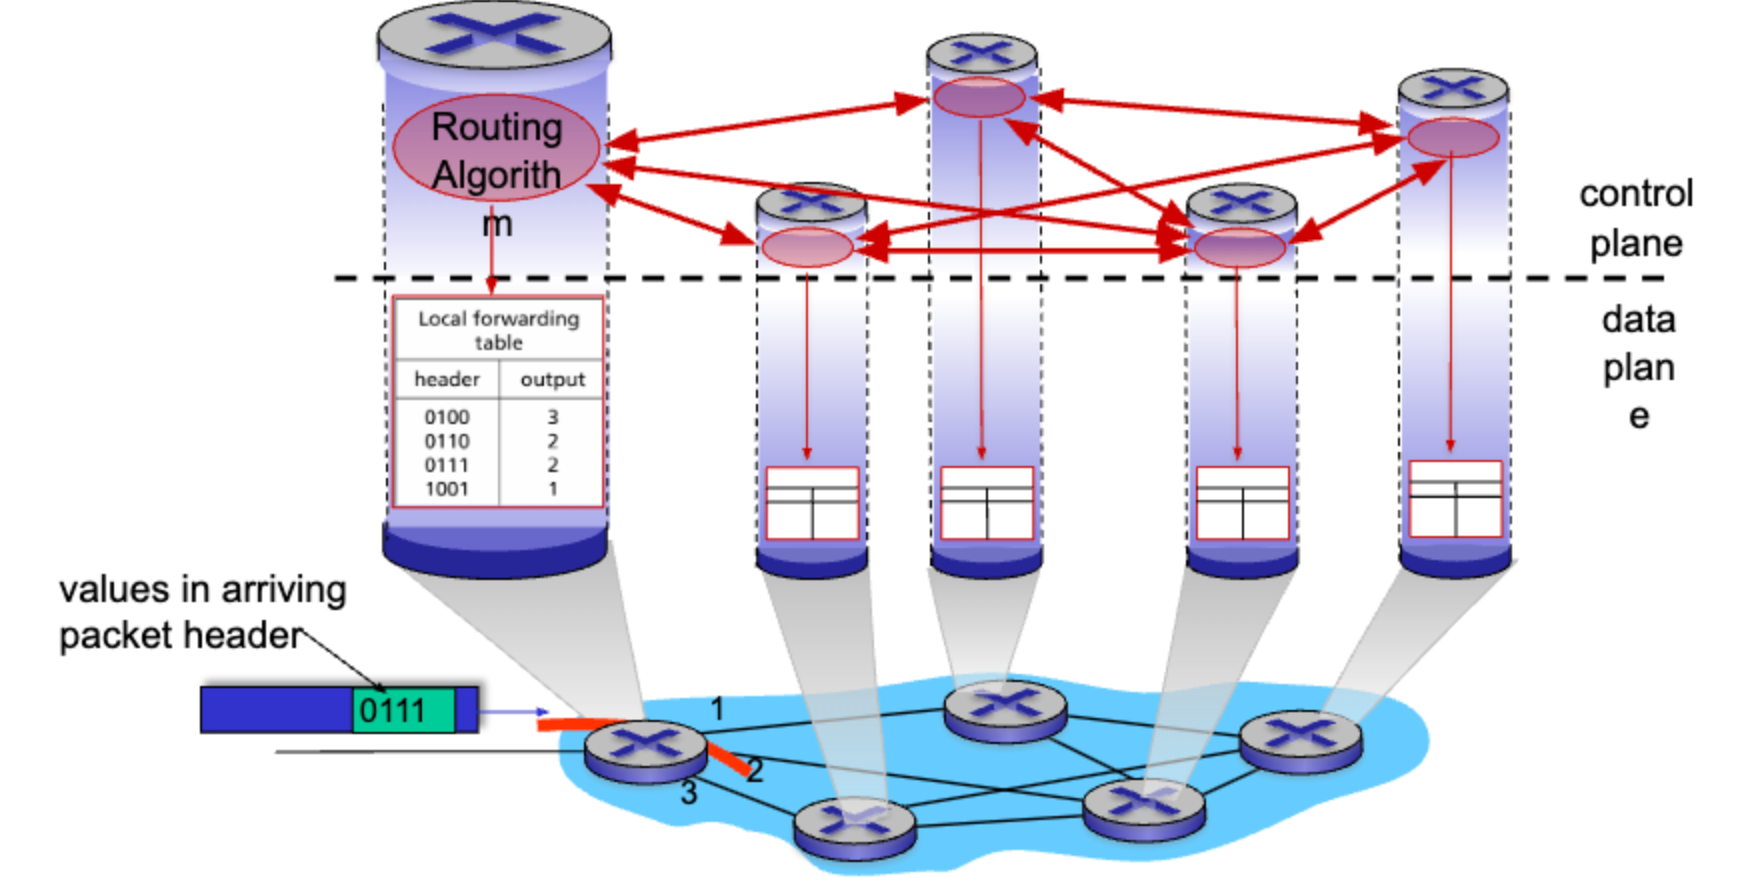
\includegraphics[width=\linewidth]{SCR-20250417-chkv.png}

	\subsection{Service Models}
	\textbf{Potential Properties:}
	\begin{itemize}
		\item Guaranteed delivery - guarantees sent packet is delivered
		\item Bounded delay - gurantees delivery within a specified delay bound
		\item In-order delivery - guarantees ordering of sent packets is consistent with ordering of recieved packets
		\item Minimum bandwidth - Guarantees delivery if packets are sent below a specified bit rate.
		\item Security - encryption at source, decruption at destination.
		\item best effort service model. \textbf{Disadvantages} - no guarantees for successful ip diagram delivery, delivery timing or order, or available bandwidth. \textbf{Advantages} - simple for wide accessibility and implementation. Good enough bandwidth. Supplemented with application layer services like datacenters and CDNs to allow services everywhere.
	\end{itemize}

	\subsection{Router}
	Allows multiple devices to communicate with each other on a network. Multiple devices can share one ip address
	\textbf{Input Ports:} Link-layer functions (hardware) \\
	\textbf{Switching Fabric:} Connects ports (hardware) \\
	\textbf{Output Ports:} Transmits packets (hardware) \\
	\textbf{Routing Processor:} Control plane (software)
	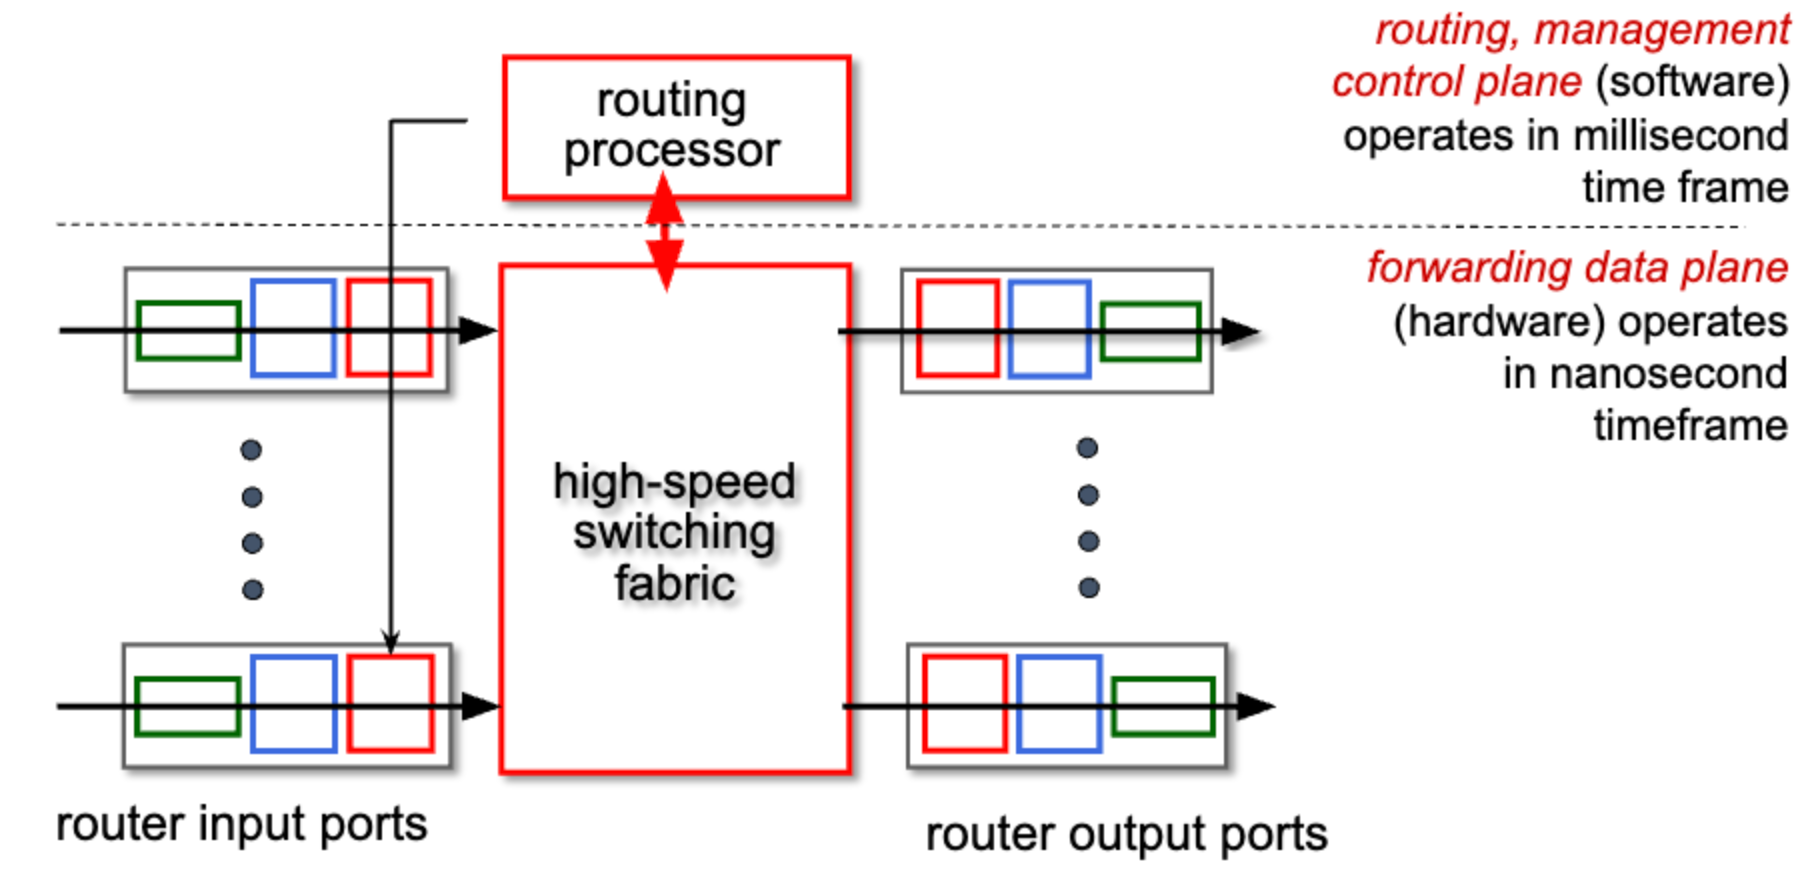
\includegraphics[width=\linewidth]{SCR-20250417-coig.png}

	\subsection{IP Datagram}
	Wraps around transport layer segments. 1-1 mapping. \\
	\textbf{Characteristics:}
	\begin{itemize}
		\item IPv4: 32-bit identifier
		\item IPv6: 128-bit identifier
		\item Assigned by ICANN
		\item Hierarchical: network ID + host ID
	\end{itemize}

	\textbf{Interface:} Connection between host/router and link \\
	\textbf{Network ID:} IP with host ID all zeros \\
	\textbf{Prefix:} Lowest IP in block + size (bits in network portion)

	\subsection{IP Support Protocols}
	\textbf{ARP:} Finds MAC for local IP \\
	\textbf{DHCP:} Dynamic IP assignment

	\textbf{IPv4}
	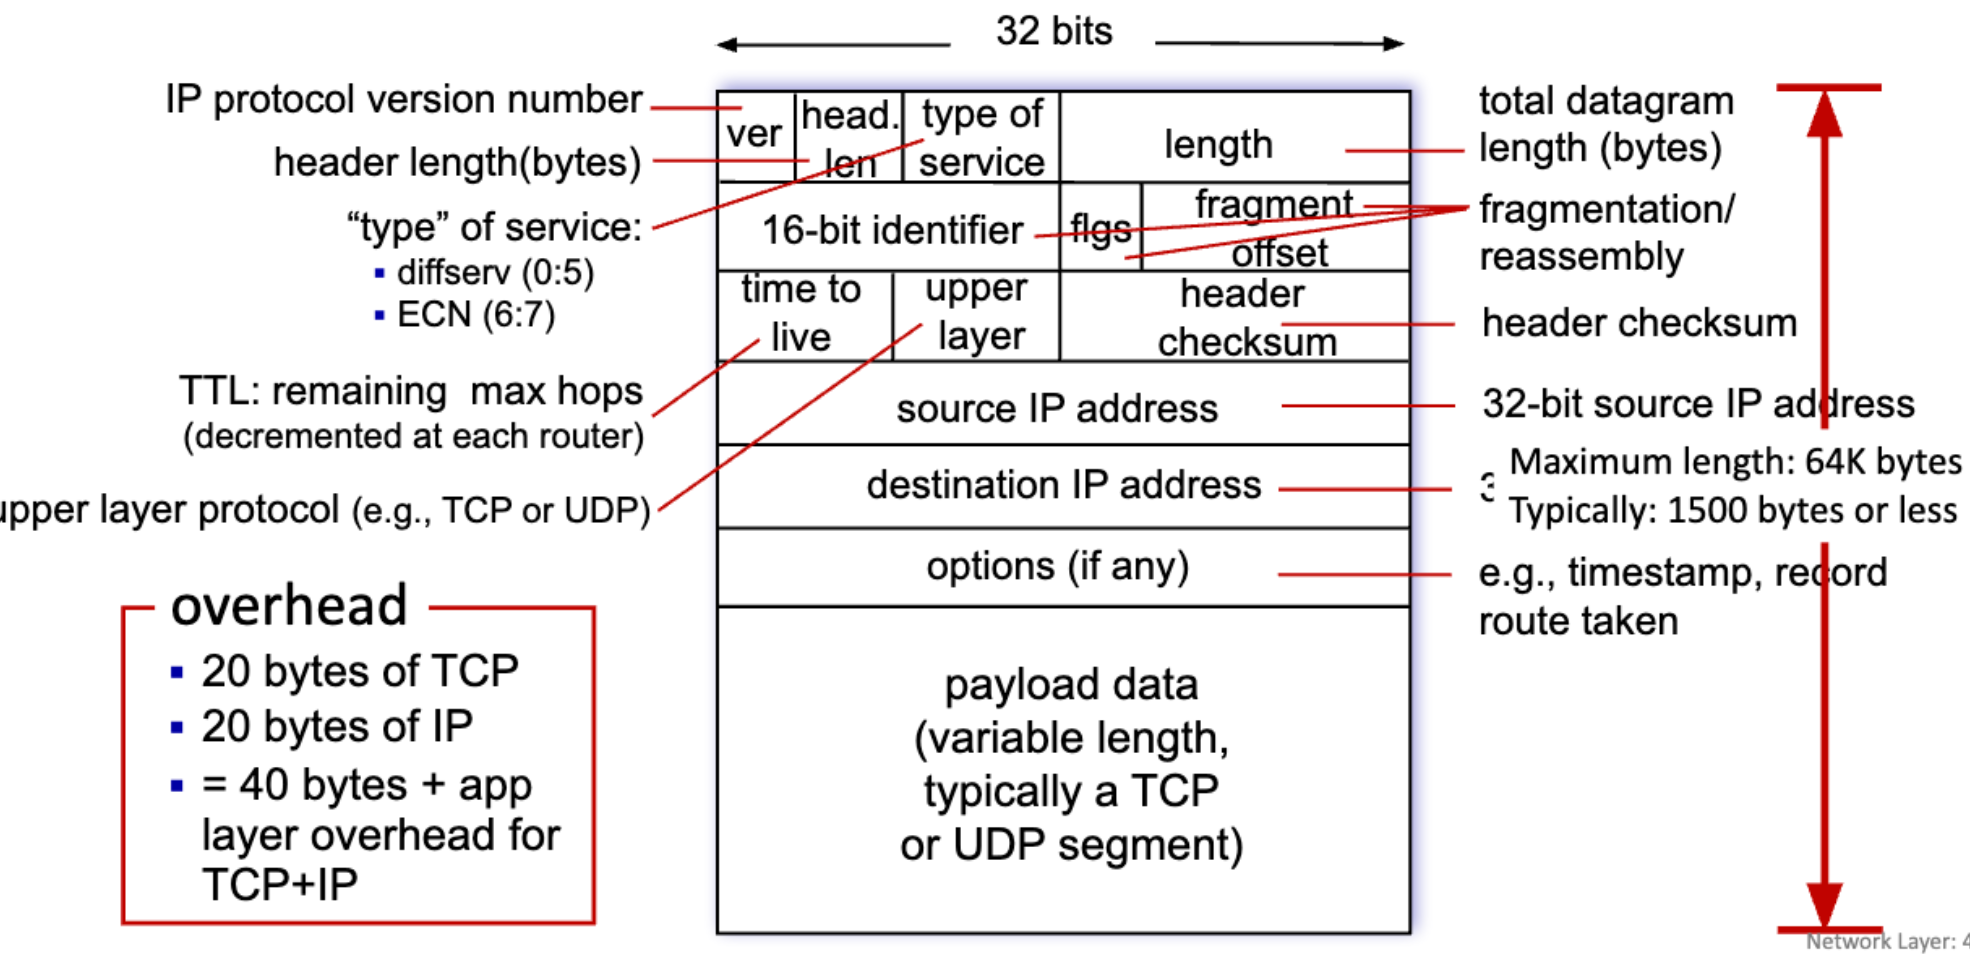
\includegraphics[width=\linewidth]{SCR-20250417-cibz.png}

	\subsection{IPv6}
	\textbf{Format:} 3fff:0000:0000:0000:0123:4567:89AB:CDEF \\
	\textbf{Shortened:} 3fff::123:4567:89AB:CDEF \\
	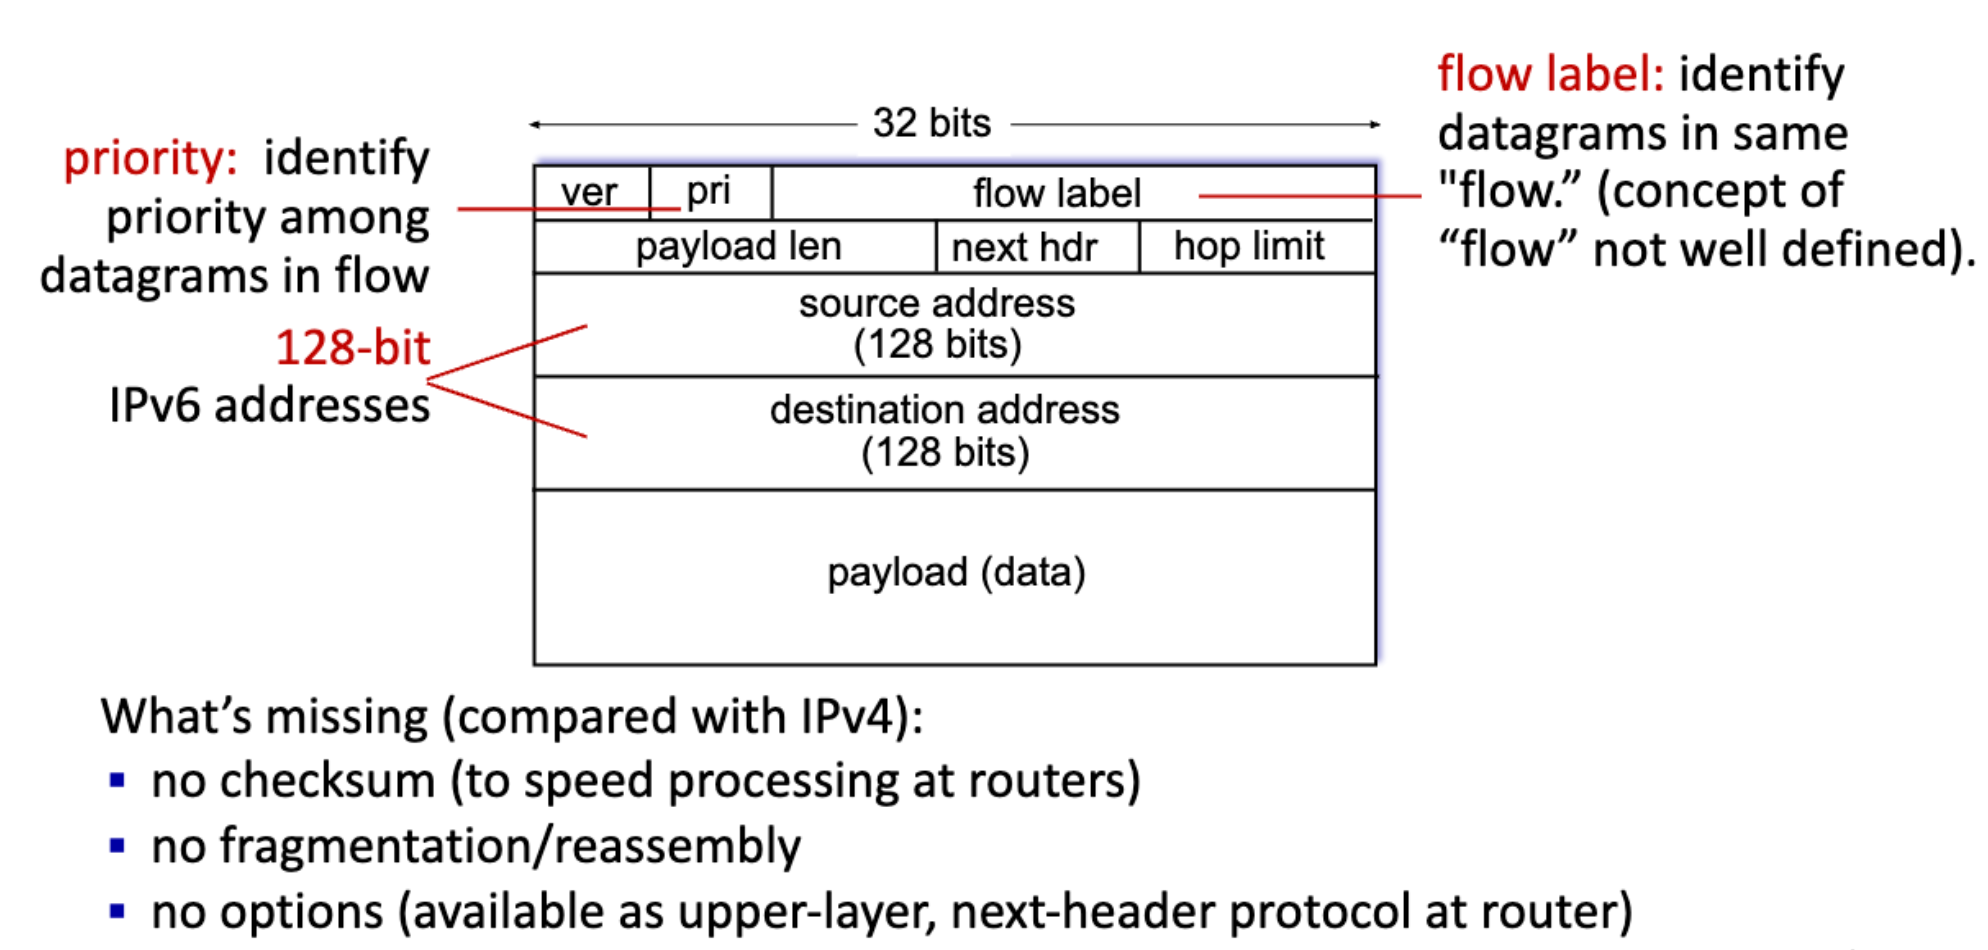
\includegraphics[width=\linewidth]{SCR-20250417-cicx.png}

	\textbf{Address Types:}
	\begin{itemize}
		\item Unicast: Single interface
		\item Anycast: Set of interfaces (closest)
		\item Multicast: Group of interfaces (all)
	\end{itemize}

	\subsection{DHCP (Dynamic Host Configuration Protocol)}
	Dynamically get IP address upon joining network. Can renew adresses, reuse addresses, and have mobile support. A \textbf{DHCP request} is encapsulated in UDP (transport layer), then IP datagram (network layer), then ethernet (link layer). \\
	\textbf{Handshake}
	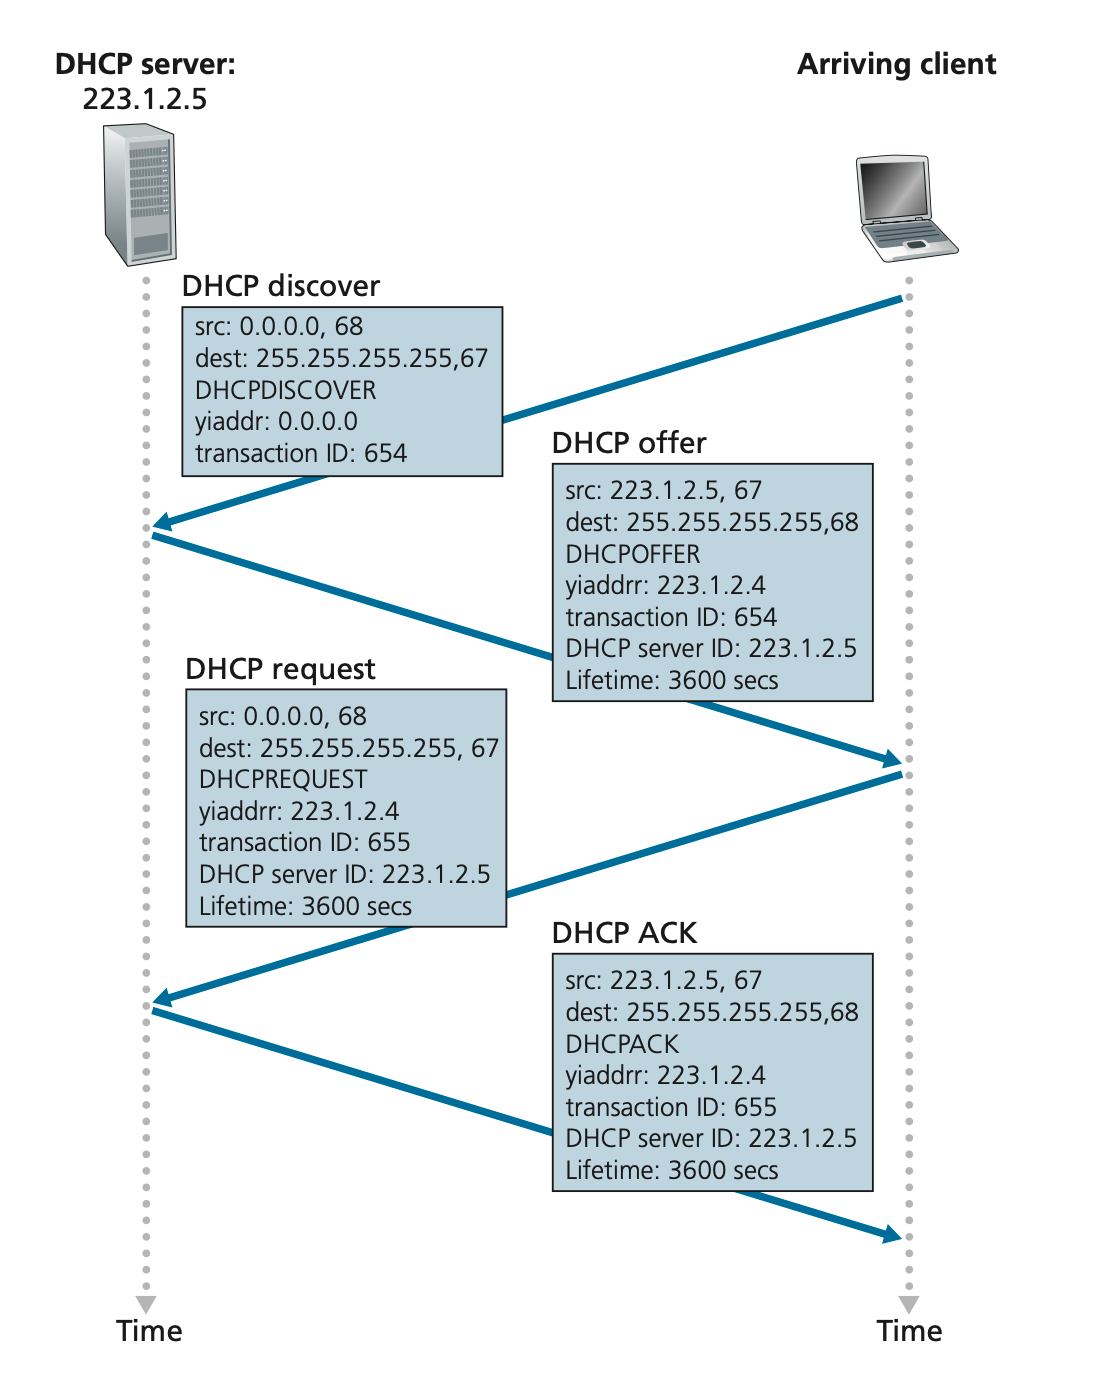
\includegraphics[width=\linewidth]{SCR-20250417-elsc.png}

	\subsection{Subnet}
	\begin{itemize}
		\item connection with direct device interface communication. (no intervening router)
		\item the blue shit in the diagram
		\item high order bits in ip addresses - common in the same subnet
		\item low order bits - unique
	\end{itemize}
	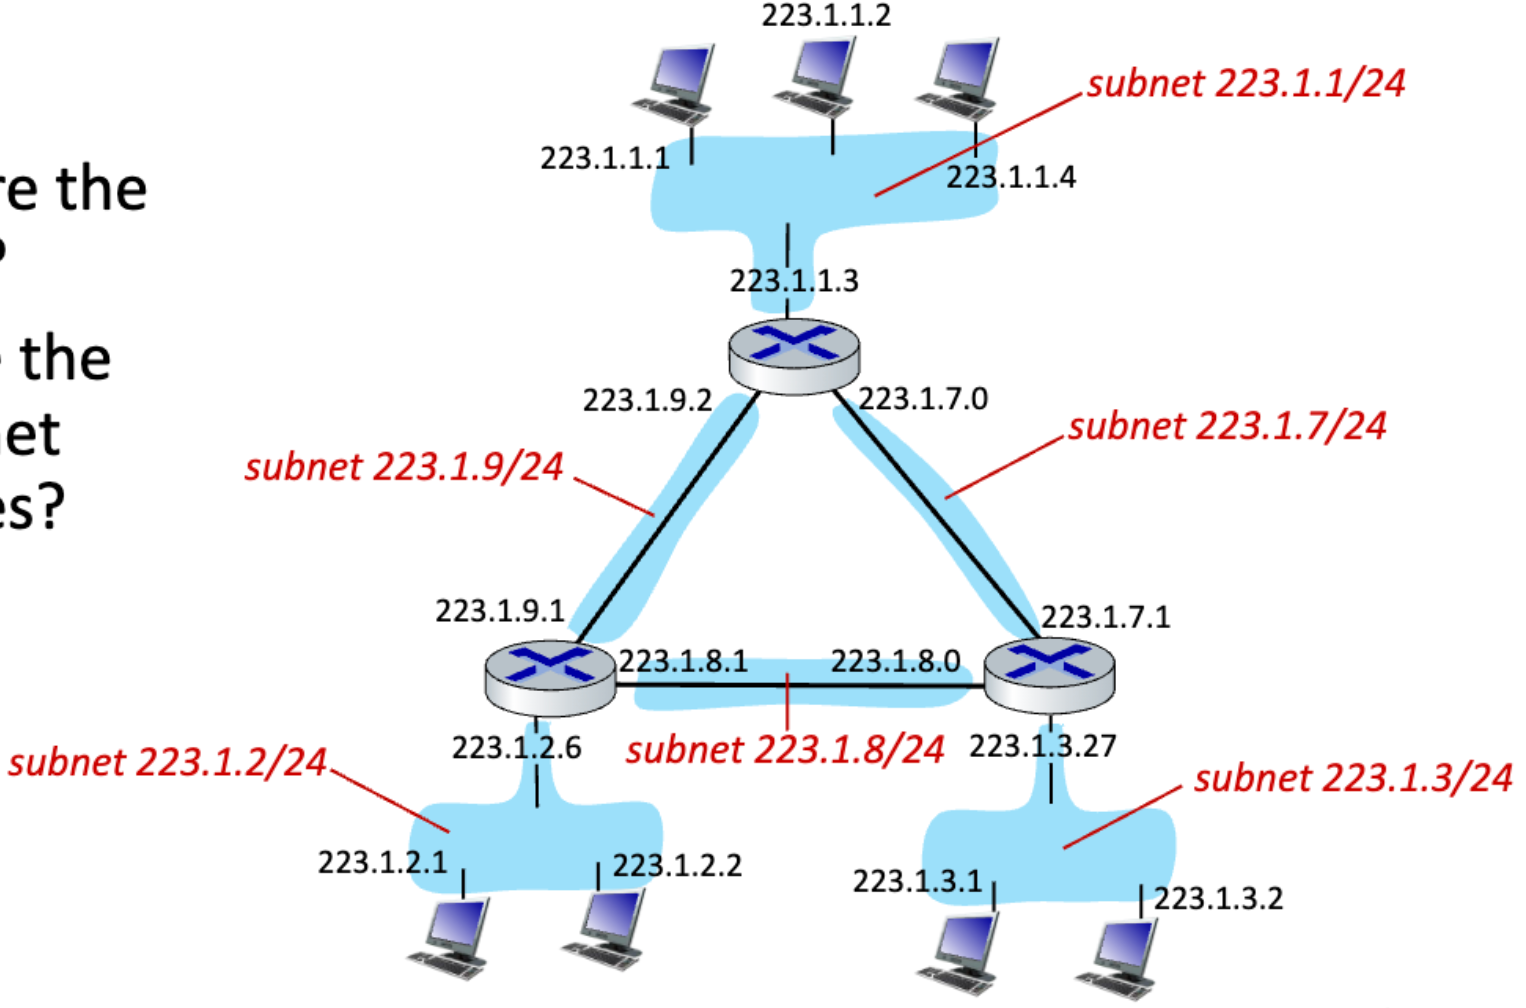
\includegraphics[width=\linewidth]{SCR-20250417-cspg.png}

	\textbf{ARP - address resolution protocol}
	Determines the mac address from the IP address.

	\subsection{ARP Protocol}
	Translates IP addresses to MAC addresses. Uses \textbf{ARP table} to store this mapping. \\
	\textbf{Algorithm}
	\begin{itemize}
		\item Sender $A$ broadcasts $B$'s ip address to every host
		\item Hosts compare, $B$ identifies it's theirs and sends its mac address towards $A$
	\end{itemize}

	\section{Link Layer}
	\subsection{Functions}
	\begin{itemize}
		\item Encapsulates network datagrams in frames
		\item Error detection/correction
		\item Link access control
		\item Reliable delivery (optional)
	\end{itemize}

	\textbf{Implementation:} Hardware (NIC) + software

	\subsection{MAC Addresses}
	Media Access Control address. Used locally to get a frame to travel across a subnet.
	\begin{itemize}
		\item 48-bit (6 bytes, 12 HEX digits)
		\item IEEE managed
		\item Typically permanent (can be spoofed)
	\end{itemize}

	\subsection{Ethernet}
	\textbf{Topologies:}
	\begin{itemize}
		\item Bus: Shared collision domain (old)
		\item Switched: Star topology with switch (current)
	\end{itemize}

	\textbf{Frame Structure:}
	\begin{itemize}
		\item Addresses: 6B source, 6B destination
		\item Type field
		\item CRC error checking
		\item Preamble (7B synchronization)
	\end{itemize}

	\textbf{Properties:} Connectionless, unreliable

	\subsection{Switch}
	\begin{itemize}
		\item Stores/forwards frames
		\item Transparent to hosts
		\item Self-learning (no configuration)
		\item Maintains switch table (MAC to interface)
	\end{itemize}

	\section{Physical Layer}
	\subsection{Signal Modulation}
	\textbf{Digital Modulation:} Converting bits to signals

	\textbf{Transmission Types:}
	\begin{itemize}
		\item Baseband: Signal occupies frequencies from zero up to a maximum (wires)
		\item Passband: Schemes that regular amplitude, phase, or frequency of carrier signal to convey bits. The signal occupies a band of frequencies around the frequency of the carrier signal. (wireless/optical)
	\end{itemize}

	\subsection{Encoding Methods}
	\textbf{NRZ:} Use a positive voltage to represent 1, negative for 0. Can use more levels of voltages, then the symbol carries more bits. Symbol rate = baud rate.\\
	\textbf{Manchester:} Mixes clock signal with data signal by XORing them together. When the clock is XORed with 0 level, it makes a low-to-high transition (logical 0). When XORed with the 1 level, it is inverted and makes a high-to-low transition (logical 1). \\
	\textbf{NRZI:}  Same as NRZ but code one as a transition and zero as no transition (or other way around). \\
	\textbf{4B/5B:}  Introduced to limit the number of consecutive 0s or 1s.  Every 4 bits mapped to a 5-bit pattern with a fixed translation table.
	% ------------- 4B/5B line‑encoding table -------------
	\textbf{4B/5B Line Encoding}

	{\renewcommand{\arraystretch}{10}% ← raise row height 25 %
		\begin{tabulary}{\linewidth}{@{}LLLL@{}} \toprule
			\textbf{Data (4B)} & \textbf{Codeword (5B)} & \textbf{Data (4B)} & \textbf{Codeword (5B)} \\ \midrule
			0000 & 11110 & 1000 & 10010 \\
			0001 & 01001 & 1001 & 10011 \\
			0010 & 10100 & 1010 & 10110 \\
			0011 & 10101 & 1011 & 10111 \\
			0100 & 01010 & 1100 & 11010 \\
			0101 & 01011 & 1101 & 11011 \\
			0110 & 01110 & 1110 & 11100 \\
			0111 & 01111 & 1111 & 11101 \\ \bottomrule
		\end{tabulary}}


	\subsection{Passband Modulation}
	\textbf{ASK:} Amplitude shift keying (different amplitudes) \\
	\textbf{FSK:} Frequency shift keying (different frequencies) \\
	\textbf{PSK:} Phase shift keying (different phases)
	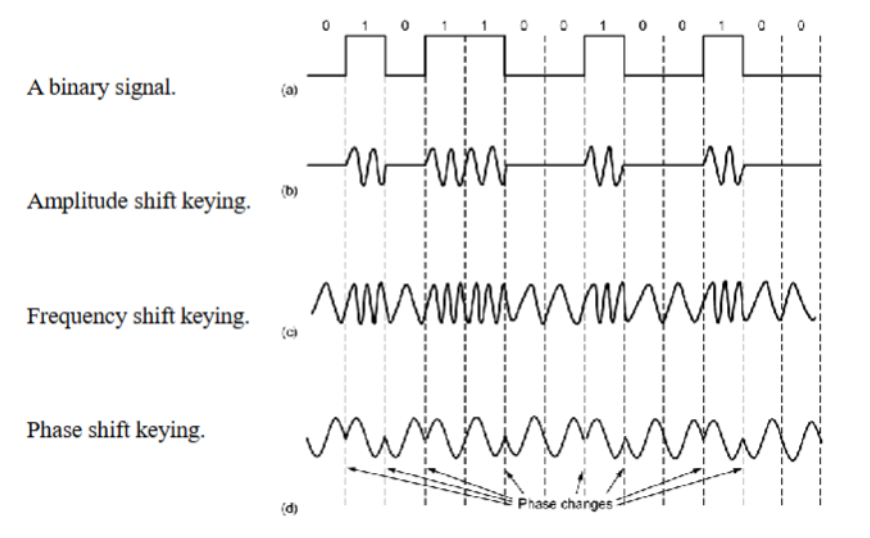
\includegraphics[width=\linewidth]{modulation.png}


	\subsection{Multiplexing}
	\textbf{TDM:} Time division multiplexing (users take turns) \\
	\textbf{FTTH:} Deployment of fiber optic cables to provide high data rates to customers. One wavelength can be shared among many houses, up to 100Mbps.
	\textbf{FDM:} Different channels transmitted in different frequency bands.
	\textbf{Cable Internet:}Internet over cable reuses the cable television plant. Data sent on a shared cable tree from head-end, not on a dedicated line per subscriber.


	\subsection{Transmission Media}
	\textbf{Guided Media:}
	\begin{itemize}
		\item Twisted Pair:
		      \begin{itemize}
			      \item Cat 5: 100Mbps (2 pairs)
			      \item Cat 5e: 1Gbps (4 pairs)
			      \item Cat 6: 10Gbps (up to 100m)
			      \item Cat 7: Shielded twisted pair
		      \end{itemize}
		\item Coaxial Cable: Better shielding, high bandwidth
		\item Power Lines: Convenient but noisy
		\item Fiber Optic: Light pulses, low error, high data rate
		      \begin{itemize}
			      \item Single-mode: Narrow, laser, long distance
			      \item Multi-mode: Wider, LED, shorter distance
		      \end{itemize}
	\end{itemize}

	\textbf{Transmission Modes:}
	\begin{itemize}
		\item Full-Duplex Link: Transmission in both directions at the same time
		\item Half-Duplex Link: Both direction transmission, but not simultaneously
		\item Simplex Link: Only one fixed direction at all times, not common
	\end{itemize}

	\textbf{Unguided Media:}
	\begin{itemize}
		\item Terrestrial wireless
		\item Satellite
		\item Laser through air
	\end{itemize}

	\subsection{Network Topologies}
	\textbf{Bus:} Single line, simple, one sender at a time \\
	\textbf{Star:} Central switch, more cabling, higher reliability, single point of failure, mutliple devies can communicate simultaneously \\
	\textbf{Ring:} Closed loop, token passing (one device at a time), difficult to expand, one computer down whole netowrk down

	\subsection{Network Hardware}
	\textbf{NIC:} Network adapter with MAC address \\
	\textbf{Hub:} All nodes receive transmissions, slow, insecure \\
	\textbf{Switch:} Only intended recipients receive data, fast, secure, plug and play \\
	\textbf{Router:} Connects LANs via IP addresses, can connect across ineternet, needs configuration \\
	\textbf{Gateway:} Connects dissimilar networks, connect coax to twisted pair.

	\subsection{Wave Properties}
	\textbf{Frequency (f):} Oscillations per second (Hz) \\
	\textbf{Period (T):} Time between maxima (sec), T = 1/f \\
	\textbf{Wavelength ($\lambda$):} Distance between maxima (m) \\
	\textbf{Relationship:} $\lambda = c/f, c \approx 3 \times 10 m/s$

	\section{Wireless Networks}
	\subsection{Types}
	\textbf{Wireless LANs:} 100ft range, WiFi (54/300/1000 Mbps) \\
	\textbf{Wide-area Wireless:} Cellular, 10's km, 1-100 Mbps

	\subsection{Characteristics}
	\textbf{Advantages:} Easy deployment, mobility support, broadcast capability \\
	\textbf{Challenges:} Interference, variable signal strength/data rates

	\section{Network Security}
	\subsection{Security Properties}
	\textbf{Confidentiality:} Only sender/receiver understand content \\
	\textbf{Message Integrity:} Content unaltered in transit \\
	\textbf{Authentication:} Verify sender/receiver identity \\
	\textbf{Operational Security:} prevent malcious attacks from public network onto private network through firewall

	\subsection{Security Concepts}
	\textbf{Firewall:} Controls access between networks \\
	\textbf{Eavesdropping:} Intercepting messages \\
	\textbf{Encryption:} Disguising data from intruders

	\textbf{Key Types:}
	\begin{itemize}
		\item Private/Symmetric: Same key for encrypt/decrypt
		\item Public/Asymmetric: Separate public/private keys
	\end{itemize}

	\subsection{Cryptographic Hash}
	Fixed-size output that's computationally infeasible to reverse or find collisions

	\textbf{Message Authentication:}
	\begin{itemize}
		\item Calculate H(m+s) where s is shared secret
		\item MAC = H(m+s)
		\item Send (m, MAC)
		\item Recipient verifies MAC
	\end{itemize}

	\subsection{Digital Signatures}
	proof of ownership of some asset they should be verifiable and the signature should not be forgable.

	\subsection{Security Layers}
	Network layer security provides blanket coverage but not user-level security
	\section{Network Security Fundamentals}

	\subsection{Core Terminology}
	\begin{itemize}
		\item \textbf{Resource:} Something valuable to the organization that must be protected.
		\item \textbf{Vulnerability:} A weakness that a threat can exploit to gain unauthorized access to a resource.
		\item \textbf{Threat:} A potential danger or circumstance that could harm a resource.
		\item \textbf{Attack:} The act of exploiting a vulnerability to compromise or steal a resource.
		\item \textbf{Risk:} The likelihood that a resource is lost, modified, or removed (\emph{Risk = Resource + Threat + Vulnerability}).
		\item \textbf{Counter‑measure:} A safeguard that mitigates a threat or reduces risk.
	\end{itemize}

	%--------------------------------------------------------------------
	\subsection{Threat‑Actor Taxonomy}
	\begin{itemize}
		\item \textbf{White‑hat:} Ethical testing, permission‐based security audits
		\item \textbf{Black‑hat:} Malicious financial or political gain
		\item \textbf{Gray‑hat:} Mix of ethical and malicious activity
		\item \textbf{Blue‑hat:} External penetration tester prior to release
		\item \textbf{Script kiddie:} Uses pre‑written exploits with minimal skill
		\item \textbf{Hacktivist:} Social or political agenda
		\item \textbf{Phreaker:} Telephony exploits for free calls or network access
		\item \textbf{Carder:} Steals and trades credit‑card data
	\end{itemize}

	%--------------------------------------------------------------------
	\subsection{Security Domains}
	\begin{itemize}
		\item \textbf{Physical Security}: Cameras, locks, controlled server‑room access.
		\item \textbf{Logical / Technical Security}: Password policy, antivirus, firewalls, VPN.
		\item \textbf{Administrative Security}: Training, phishing simulations, data‑leak prevention.
	\end{itemize}

	%====================================================================
	\section{Threat Landscape}

	\subsection{Network Threats}
	\textbf{Malware Types:}
	\begin{itemize}
		\item Virus – self‑replicating; needs user activation
		\item Worm – self‑replicating; auto‑spreads without user action
		\item Spyware – covertly monitors users
		\item Adware – injects unwanted advertisements
		\item Scareware – fake security warnings to provoke action
		\item Trojan – legitimate‑looking program with hidden payload
		\item Ransomware – encrypts data until ransom is paid
	\end{itemize}

	%--------------------------------------------------------------------
	\subsection{Attack Types}
	\textbf{Reconnaissance (Passive):}
	\begin{itemize}
		\item Ping Sweep – identify live hosts
		\item Port Scanning – discover open services
		\item Packet Sniffing – capture and inspect traffic
	\end{itemize}

	\textbf{Access Attacks:}
	\begin{itemize}
		\item Phishing – deceptive e‑mails / sites for credentials
		\item Pharming – DNS / hosts‑file redirection
		\item MITM – intercept traffic
		      \begin{itemize}
			      \item Spoofing – falsify source identity
			      \item Hijacking – take over authenticated session
		      \end{itemize}
	\end{itemize}

	\textbf{Denial‑of‑Service (DoS):}
	\begin{itemize}
		\item Saturation Flood – overwhelm with requests
		\item Vulnerability Exploitation – crash service via bug
	\end{itemize}

	\textbf{Distributed DoS (DDoS) Examples:}
	\begin{itemize}
		\item SYN Flood – half‑open TCP handshakes
		\item ICMP Flood – excessive echo/response traffic
	\end{itemize}

	%--------------------------------------------------------------------
	\subsection{Security Best Practices}
	\begin{itemize}
		\item Segmentation / security zones
		\item Defense‑in‑depth (layered controls)
		\item Least‑privilege access
		\item Adequate protection at every OSI layer
		\item Information‑access restriction
		\item Separation of duties \& job rotation
	\end{itemize}

	\subsection{Security Measures by Goal}
	\begin{itemize}
		\item \textbf{Preventive} – firewalls, locks, policies
		\item \textbf{Detective} – logs, IDS/IPS, CCTV
		\item \textbf{Corrective} – patching, configuration fixes
		\item \textbf{Recovery} – backups, system restore
		\item \textbf{Deterrent} – legal notices, sanctions
	\end{itemize}

	\subsection{Protocol Summary by Layer}

	\textbf{Application:} DNS (53), HTTP (80), HTTPS (443), SMTP (25), POP3 (110), IMAP (143), FTP (20/21), TELNET (23), SSH (22), DHCP (67/68), RTP, VoIP, SSL/TLS, MPEG-4, H.264, HTML5, CSS

	\textbf{Transport:} TCP, UDP

	\textbf{Network:} IP, ICMP, ARP, IPX, AppleTalk, OSPF, BGP, RIP, MPLS-VPN, EVPN

	\textbf{Link:} Ethernet (802.3), Wi-Fi (802.11), Token Ring (802.5), Bluetooth, Zigbee, Frame Relay, CSMA/CD, Token passing

	\textbf{Physical:} ADSL (G.992), Coaxial cable, Twisted pair copper, Fiber optic, Wireless transmission media

\end{multicols*}

\end{document}